% TODO checklist:
% - [x] Inspected src/mcp/tools/ directory structure (17 categories)
% - [x] Inspected src/mcp/tools/README_mcp_tools.md (all 34 tools documented)
% - [x] Inspected Q&A.md Q37 for tool inventory and categorization
% - [x] Inspected individual tool implementations for capabilities
% - [x] Cross-referenced with sapthesis-doc.tex subsection on Tool Inventory Summary

\section{Tool Categories and Inventory}
\label{sec:tool-inventory}

The Cineca Agentic Platform implements 34 MCP tools organized into 17 categories. Each category groups related functionality and shares common security scopes and operational characteristics. This section provides a comprehensive inventory of all tools, their actions, and their roles within the platform.

\subsection{Category Organization}
\label{subsec:category-organization}

Tools are organized in a two-level hierarchy: \textit{category} and \textit{tool}. The category represents a functional domain (e.g., \texttt{graph}, \texttt{security}), while the tool represents a specific capability within that domain (e.g., \texttt{graph.query}, \texttt{security.audit}).

\begin{figure}[htbp]
    \centering
    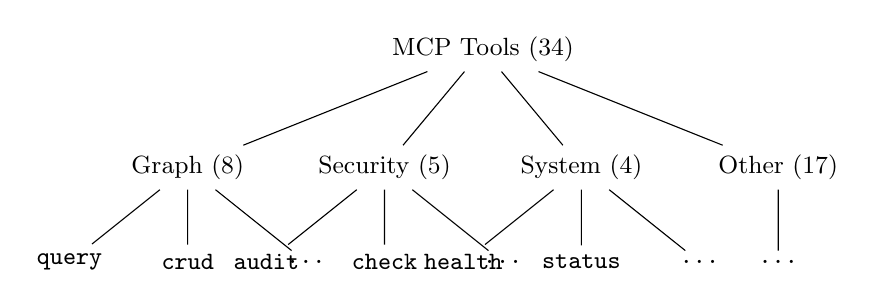
\begin{tikzpicture}[
        level 1/.style={sibling distance=2.5cm, level distance=1.5cm},
        level 2/.style={sibling distance=1.5cm, level distance=1.2cm},
        every node/.style={font=\small}
    ]
        \node {MCP Tools (34)}
            child { node {Graph (8)}
                child { node {\texttt{query}} }
                child { node {\texttt{crud}} }
                child { node {\texttt{...}} }
            }
            child { node {Security (5)}
                child { node {\texttt{audit}} }
                child { node {\texttt{check}} }
                child { node {\texttt{...}} }
            }
            child { node {System (4)}
                child { node {\texttt{health}} }
                child { node {\texttt{status}} }
                child { node {\texttt{...}} }
            }
            child { node {Other (17)}
                child { node {\texttt{...}} }
            };
    \end{tikzpicture}
    \caption{Hierarchical organization of MCP tools by category.}
    \label{fig:tool-hierarchy}
\end{figure}

\subsection{Tool Inventory Summary}
\label{subsec:tool-inventory-summary}

Table~\ref{tab:tool-inventory} provides a complete inventory of all 34 tools with their categories, primary actions, and required scopes. Detailed specifications for each tool are provided in Appendix~B (MCP Tool Reference).

\begin{longtable}{llp{4cm}l}
    \caption{Complete MCP tool inventory with categories and scopes}
    \label{tab:tool-inventory} \\
    \toprule
    \textbf{Tool Name} & \textbf{Category} & \textbf{Actions} & \textbf{Required Scope} \\
    \midrule
    \endfirsthead
    \multicolumn{4}{c}{\tablename\ \thetable\ -- \textit{Continued from previous page}} \\
    \toprule
    \textbf{Tool Name} & \textbf{Category} & \textbf{Actions} & \textbf{Required Scope} \\
    \midrule
    \endhead
    \midrule
    \multicolumn{4}{r}{\textit{Continued on next page}} \\
    \endfoot
    \bottomrule
    \endlastfoot
    % Graph Tools
    \texttt{graph.query} & Graph & run, explain, profile & \texttt{graph:read} \\
    \texttt{graph.secure\_query} & Graph & query, explain & \texttt{graph:read} \\
    \texttt{graph.search} & Graph & search\_nodes, search\_edges, fulltext & \texttt{graph:read} \\
    \texttt{graph.schema} & Graph & get\_schema, list\_labels, list\_rels & \texttt{graph:read} \\
    \texttt{graph.analytics} & Graph & centrality, communities, paths & \texttt{graph:read} \\
    \texttt{graph.crud} & Graph & create, read, update, delete & \texttt{graph:write} \\
    \texttt{graph.bulk} & Graph & create\_nodes, create\_edges, delete & \texttt{graph:write} \\
    \texttt{graph.generate\_cypher} & Graph & generate, validate, explain & \texttt{graph:read} \\
    \midrule
    % Security Tools
    \texttt{security.check} & Security & validate\_config, check\_perms & \texttt{security:admin} \\
    \texttt{security.audit} & Security & log, query, export & \texttt{security:audit} \\
    \texttt{security.permissions} & Security & check, list\_policies, evaluate & \texttt{security:read} \\
    \texttt{security.allowed\_ops} & Security & list & \texttt{security:read} \\
    \texttt{security.describe\_principal} & Security & describe & \texttt{security:read} \\
    \midrule
    % System Tools
    \texttt{system.health} & System & liveness, readiness, details & \texttt{tools:read} \\
    \texttt{system.status} & System & status & \texttt{tools:read} \\
    \texttt{system.metrics} & System & scrape, info & \texttt{tools:read} \\
    \texttt{system.backup} & System & create, list, restore, delete & \texttt{system:admin} \\
    \midrule
    % Model Tools
    \texttt{model.manage} & Model & list, switch, status, configure & \texttt{model:admin} \\
    \texttt{model.test} & Model & test\_completion, benchmark & \texttt{model:read} \\
    \midrule
    % Output Tools
    \texttt{output.format} & Output & json, csv, markdown, text & \texttt{tools:read} \\
    \texttt{output.summarize} & Output & extractive, abstractive, keywords & \texttt{tools:read} \\
    \midrule
    % Data Tools
    \texttt{data.archive} & Data & archive\_nodes, restore, purge & \texttt{data:admin} \\
    \texttt{data.quality} & Data & check\_integrity, find\_orphans & \texttt{data:read} \\
    \midrule
    % Agent Tools
    \texttt{agent.context} & Agent & assemble & \texttt{tools:read} \\
    \midrule
    % Cache Tools
    \texttt{cache.manage} & Cache & get, set, delete, keys, ttl & \texttt{tools:write} \\
    \midrule
    % Catalog Tools
    \texttt{catalog.discover} & Catalog & list, describe, search & \texttt{tools:read} \\
    \midrule
    % DB Tools
    \texttt{db.switch} & Database & switch, list, status & \texttt{db:admin} \\
    \midrule
    % Errors Tools
    \texttt{errors.report} & Errors & report, list, details & \texttt{tools:read} \\
    \midrule
    % Privacy Tools
    \texttt{privacy.consent} & Privacy & get, set, revoke, audit & \texttt{privacy:admin} \\
    \midrule
    % Rate Limit Tools
    \texttt{ratelimit.manage} & Rate Limit & get\_limits, set\_limits, reset & \texttt{ratelimit:admin} \\
    \midrule
    % Session Tools
    \texttt{session.manage} & Session & create, get, update, delete, extend & \texttt{session:write} \\
    \midrule
    % Tenancy Tools
    \texttt{tenancy.manage} & Tenancy & list, current, switch, create, delete & \texttt{tools:admin} \\
    \midrule
    % User Tools
    \texttt{user.profile} & User & get, set, update, delete & \texttt{tools:user} \\
    \midrule
    % Viz Tools
    \texttt{viz.render} & Visualization & render\_graph, render\_table, sparkline & \texttt{viz:render} \\
\end{longtable}

\subsection{Graph Tools}
\label{subsec:graph-tools}

Graph tools provide comprehensive access to the Memgraph knowledge graph, supporting both read operations and write mutations. These tools are the most heavily used in agent workflows, particularly for natural language question-answering.

\subsubsection{\texttt{graph.query}: Direct Cypher Execution}

The \texttt{graph.query} tool executes Cypher queries directly against Memgraph. It is designed for advanced users and internal orchestrator use where the Cypher is already validated.

\paragraph{Actions.}
\begin{itemize}
    \item \texttt{run}: Execute Cypher query and return results.
    \item \texttt{explain}: Return query execution plan without executing.
    \item \texttt{profile}: Execute query and return performance profile.
\end{itemize}

\paragraph{Safety Features.}
\begin{itemize}
    \item \textbf{Read-only mode}: When \texttt{read\_only=true}, write operations are blocked at the query level.
    \item \textbf{Timeout}: Per-query timeout prevents runaway queries.
    \item \textbf{Row limiting}: Client-side result slicing prevents memory exhaustion.
\end{itemize}

\begin{lstlisting}[language=Python, caption={graph.query tool usage example}, label={lst:graph-query-example}]
result = invoke("graph.query", {
    "action": "run",
    "cypher": "MATCH (p:Person)-[:WORKS_AT]->(o:Org) RETURN p.name, o.name LIMIT 10",
    "params": {},
    "read_only": True,
    "timeout_ms": 5000,
    "limit": 100
})
# Returns: {"ok": true, "columns": ["p.name", "o.name"], "rows": [...], "rowcount": 10}
\end{lstlisting}

\subsubsection{\texttt{graph.secure\_query}: NL-to-Cypher with Validation}

The \texttt{graph.secure\_query} tool provides the end-to-end NL-to-Cypher pipeline with safety validation. It is the primary interface for natural language graph queries.

\paragraph{Actions.}
\begin{itemize}
    \item \texttt{query}: Convert natural language to Cypher and execute.
    \item \texttt{explain}: Return generated Cypher without execution.
\end{itemize}

\paragraph{Pipeline.}
\begin{enumerate}
    \item Natural language question is received.
    \item Graph schema is retrieved for context.
    \item LLM generates Cypher query.
    \item Query is validated for safety (no writes, bounded complexity).
    \item Validated query is executed.
    \item Results are returned with the generated Cypher.
\end{enumerate}

\subsubsection{\texttt{graph.schema}: Schema Introspection}

The \texttt{graph.schema} tool provides metadata about the graph structure, essential for NL-to-Cypher context and data modeling.

\paragraph{Actions.}
\begin{itemize}
    \item \texttt{get\_schema}: Return complete schema with labels, relationships, and properties.
    \item \texttt{list\_labels}: Return all node labels.
    \item \texttt{list\_relationships}: Return all relationship types.
    \item \texttt{get\_constraints}: Return schema constraints and indexes.
\end{itemize}

\subsubsection{\texttt{graph.analytics}: Graph Algorithms}

The \texttt{graph.analytics} tool exposes graph analytics algorithms with bounded computation to prevent resource exhaustion.

\paragraph{Actions.}
\begin{itemize}
    \item \texttt{centrality}: Calculate degree, betweenness, or PageRank centrality.
    \item \texttt{communities}: Detect communities using Louvain or label propagation.
    \item \texttt{paths}: Find all paths between two nodes.
    \item \texttt{shortest\_path}: Calculate shortest path with optional weighting.
\end{itemize}

\paragraph{Resource Bounds.}
All analytics operations are bounded by:
\begin{itemize}
    \item Maximum result limit (default: 1000 nodes).
    \item Computation timeout (default: 30 seconds).
    \item Memory limits for intermediate results.
\end{itemize}

\subsubsection{\texttt{graph.crud} and \texttt{graph.bulk}: Write Operations}

Write tools provide transactional modifications to the graph with full audit logging.

\paragraph{\texttt{graph.crud} Actions.}
\begin{itemize}
    \item \texttt{create\_node}: Create a single node with labels and properties.
    \item \texttt{read\_node}: Read a node by ID.
    \item \texttt{update\_node}: Update node properties.
    \item \texttt{delete\_node}: Soft or hard delete a node.
    \item Equivalent actions for edges.
\end{itemize}

\paragraph{\texttt{graph.bulk} Features.}
\begin{itemize}
    \item Batch operations for multiple nodes/edges.
    \item Idempotency keys to prevent duplicate creation on retry.
    \item Transactional execution (all-or-nothing).
    \item Progress reporting for large batches.
\end{itemize}

\subsection{Security Tools}
\label{subsec:security-tools}

Security tools provide introspection and management of the platform's security controls.

\subsubsection{\texttt{security.audit}: Audit Log Access}

The \texttt{security.audit} tool provides programmatic access to the audit trail.

\paragraph{Actions.}
\begin{itemize}
    \item \texttt{log}: Record a custom audit event.
    \item \texttt{query}: Search audit logs with filters.
    \item \texttt{export}: Export audit logs for compliance.
\end{itemize}

\subsubsection{\texttt{security.permissions}: Permission Checking}

The \texttt{security.permissions} tool allows runtime permission evaluation.

\paragraph{Actions.}
\begin{itemize}
    \item \texttt{check}: Verify if a permission is granted for a resource.
    \item \texttt{list\_policies}: List policies applicable to the current principal.
    \item \texttt{evaluate}: Evaluate a permission with full context (ABAC).
\end{itemize}

\subsubsection{\texttt{security.describe\_principal}: Identity Introspection}

The \texttt{security.describe\_principal} tool returns details about the current authenticated principal.

\paragraph{Response.}
\begin{lstlisting}[language=Python, caption={Principal description response}, label={lst:principal-describe}]
{
    "ok": true,
    "principal": {
        "id": "user_123",
        "type": "user",
        "tenant": "tenant_abc",
        "groups": ["users", "researchers"],
        "permissions": ["graph:read", "tools:basic", "user:me"],
        "token_exp": "2025-01-15T12:00:00Z"
    }
}
\end{lstlisting}

\subsection{System Tools}
\label{subsec:system-tools}

System tools provide operational visibility and management capabilities.

\subsubsection{\texttt{system.health}: Health Probes}

The \texttt{system.health} tool implements Kubernetes-compatible health probes.

\paragraph{Actions.}
\begin{itemize}
    \item \texttt{liveness}: Quick self-check (is the process alive?).
    \item \texttt{readiness}: Dependency checks (are backends reachable?).
    \item \texttt{details}: Readiness with version and environment information.
\end{itemize}

\paragraph{Component Checks.}
\begin{lstlisting}[language=Python, caption={Health check response with component details}, label={lst:health-response}]
{
    "ok": true,
    "action": "readiness",
    "checked_at": "2025-01-15T10:30:00Z",
    "summary": {"passed": 3, "failed": 0, "skipped": 0},
    "components": {
        "app": {"status": "up", "latency_ms": 0.5},
        "db": {"status": "up", "latency_ms": 12.3},
        "redis": {"status": "up", "latency_ms": 2.1}
    }
}
\end{lstlisting}

\subsubsection{\texttt{system.backup}: Backup Management}

The \texttt{system.backup} tool manages graph and system backups.

\paragraph{Actions.}
\begin{itemize}
    \item \texttt{create}: Create a new backup with optional compression.
    \item \texttt{list}: List available backups.
    \item \texttt{restore}: Restore from a backup.
    \item \texttt{delete}: Delete old backups.
    \item \texttt{export/import}: Data migration operations.
\end{itemize}

\subsection{Model Tools}
\label{subsec:model-tools}

Model tools provide runtime LLM management and testing capabilities.

\subsubsection{\texttt{model.manage}: Model Configuration}

The \texttt{model.manage} tool allows switching between LLM models and configuring parameters.

\paragraph{Actions.}
\begin{itemize}
    \item \texttt{list}: List available models with their status.
    \item \texttt{switch}: Change the active model for subsequent operations.
    \item \texttt{status}: Get current model configuration.
    \item \texttt{configure}: Update model parameters (temperature, max\_tokens).
\end{itemize}

\subsubsection{\texttt{model.test}: Model Testing}

The \texttt{model.test} tool provides lightweight LLM testing capabilities.

\paragraph{Actions.}
\begin{itemize}
    \item \texttt{test\_completion}: Test text completion with optional simulation mode.
    \item \texttt{test\_embedding}: Test embedding generation.
    \item \texttt{benchmark}: Run performance benchmarks.
\end{itemize}

\subsection{Other Tool Categories}
\label{subsec:other-tools}

The remaining tool categories provide specialized functionality:

\begin{description}
    \item[Agent (\texttt{agent.context})] Assembles execution context from sessions, preferences, and history.
    
    \item[Cache (\texttt{cache.manage})] Redis-backed caching with tenant namespacing and TTL support.
    
    \item[Catalog (\texttt{catalog.discover})] Tool discovery and metadata retrieval for dynamic tool selection.
    
    \item[Data (\texttt{data.archive}, \texttt{data.quality})] Data archival with soft-delete semantics and quality validation.
    
    \item[Database (\texttt{db.switch})] Database connection management for multi-database environments.
    
    \item[Errors (\texttt{errors.report})] Structured error reporting with PII sanitization.
    
    \item[Output (\texttt{output.format}, \texttt{output.summarize})] Result formatting and text summarization.
    
    \item[Privacy (\texttt{privacy.consent})] User consent registry with audit trail.
    
    \item[Rate Limit (\texttt{ratelimit.manage})] Rate limit configuration and monitoring.
    
    \item[Session (\texttt{session.manage})] Session lifecycle with TTL enforcement.
    
    \item[Tenancy (\texttt{tenancy.manage})] Tenant administration with soft-delete protection.
    
    \item[User (\texttt{user.profile})] User preferences and profile storage with JSONB semantics.
    
    \item[Visualization (\texttt{viz.render})] Graph visualization (Mermaid/DOT) and data rendering.
\end{description}

\subsection{Tool Discovery Mechanism}
\label{subsec:discovery-mechanism}

The platform provides multiple mechanisms for tool discovery:

\paragraph{REST API Discovery.}
\begin{lstlisting}[language=Python, caption={Tool discovery via REST API}, label={lst:rest-discovery}]
# List all tools
GET /v1/tools
# Response: {"tools": [...], "total": 34, "categories": [...]}

# Get tool schema
GET /v1/tools/graph.query/schema
# Response: {"name": "graph.query", "actions": [...], "schema": {...}}
\end{lstlisting}

\paragraph{Programmatic Discovery.}
\begin{lstlisting}[language=Python, caption={Tool discovery via catalog.discover}, label={lst:programmatic-discovery}]
# From within an agent run
result = invoke("catalog.discover", {
    "action": "list",
    "category": "graph",
    "include_schema": True
})

# Search by capability
result = invoke("catalog.discover", {
    "action": "search",
    "query": "query graph",
    "include_examples": True
})
\end{lstlisting}

\paragraph{Auto-Registration.}
Tools are automatically discovered through the module naming convention. Any Python module under \texttt{src/mcp/tools/<category>/<tool>.py} that exposes an \texttt{invoke}, \texttt{run}, or \texttt{handle} function is automatically registered without explicit configuration.

\subsection{Summary}
\label{subsec:inventory-summary}

The MCP tools ecosystem provides comprehensive coverage of platform functionality:

\begin{itemize}
    \item \textbf{34 tools} across \textbf{17 categories}.
    \item \textbf{Graph tools} (8) form the core for knowledge graph interactions.
    \item \textbf{Security tools} (5) provide introspection and audit capabilities.
    \item \textbf{System tools} (4) enable operational monitoring and management.
    \item \textbf{Specialized tools} (17) cover caching, sessions, tenancy, and more.
    \item \textbf{Automatic discovery} eliminates manual registration overhead.
    \item \textbf{Scope-based access} ensures proper authorization for each tool.
\end{itemize}

This comprehensive tooling layer enables agents to perform complex tasks while maintaining security, observability, and governance requirements.
